% BENCHMARKING
\section{Benchmarking}

Due to modification of the {\bf Mineos} codes, the revised version has been
benchmarked again. Three benchmark tests were performed:
test against the original code at UCSD, test against Bob Hermann's
eigenfunction and synthetic seismogram code for fundamental modes, 
and test against SPECFEM3D\_GLOBE v3.6 code designed for
simulation of three-dimensional global seismic wave propagation
based upon the spectral-element method (SEM).

\subsection{Benchmark test \#1. Revised version vs UCSD version.}

This test consists of computation  by both codes of eigenvalues and 
eigenfunctions for all types of oscillation (spheroidal, toroidal, 
inner core toroidal, and radial), and, finally, synthetic seismograms for 
spheroidal, toroidal and radial oscillations.
Eigenvalues and eigenfunctions  were computed for the first four branches
($n=0,1,2,3$) in the frequency range from zero to 0.25 Hz. 
The test showed a perfect matching of the eigenvalues, eigenfunctions and 
synthetic seismograms for both codes. Differences did not exceed the last 
significant digit. The most important difference of the revised version against
the UCSD code is that the revised code uses sensor orientation ``Up" instead 
of ``Down". The revised code uses  the coordinate system ``Up", ``South", and
``East", so we need to reverse the sign of all Green functions and synthetic
seismograms of the UCSD code to get the revised code results.
Also note that the revised {\bf Mineos} version uses geographic coordinates 
for the input data; i.e, station and event locations, instead of geocentric 
ones as in the old version. {\bf Mineos} automatically converts geographic 
coordinates to geocentric for internal computations.

\subsection{Benchmark test \#2. Mineos code vs plane Herrmann's code
for fundamental modes}
The {\bf Mineos} synthetic seismograms were benchmarked against Herrmann's plane
code seismograms for the fundamental spheroidal and toroidal modes in the period range 
6 - 100 seconds. For testing purposes, there were taken 8 1D models: 
6 vertical profiles of the global 3D CUB2.0 CU Earth model, PREM
model with 3 km water layer, and PREM model with water layer filled with
upper crust. The chosen 6 points are located at
places characterized by different tectonics, namely:
\begin{itemize}
\item Korean Peninsula, (36N, 128E);
\item Uta, USA, seismo-tectonic region, (40N, 112W);
\item near Hudson bay, Cananda, craton, (56N, 90W);
\item center of Hudson Bay, Canada, craton, (58N, 86N);
\item young Pacific Ocean, (0N, 100W);
\item old Pacific Ocean, (40N, 160E).
\end{itemize}
To take into account the Earth's sphericity, the original version of the 
Herrmann's plane code (Herrmann, 1978) had been modified using the Earth 
flattening exact formulas for Love waves (Biswas \& Knopoff, 1970) and Earth 
flattening approximation for Rayleigh waves (Biswas, 1972). All input
information in Herrmann's code is in geocentric coordinates.

\noindent As an example, Figures \ref{fig:1a} - \ref{fig:3a} illustrate plane 
(blue) and spherical (red) 
three-component synthetic seismogram for the three different seismic stations: 
BJT, TLY, and BILL.
The event location (CMT solution) is (25.39N, 101.40E), depth is 33 km.
The station coordinates (geographic),  epicentral distances (geocentric), 
and source azimuths (geocentric) are shown in the Table 1;  units are degrees.

\begin{center}
\begin{tabular}{|c|c|r|r|r|r|}
\multicolumn{5}{c}{{\bf Table 1.}}  \\ \hline
Cod & Station name & Latitude & Longitude & Distance & Azimuth \\ \cline{1-6}
BJT & \multicolumn{1}{l|}{{Beijing, China}} & 40.0183N & 116.1679E & 19.123 & -135.267 \\
TLY & \multicolumn{1}{l|}{{Talaya, Russia}} & 51.6807N & 103.6438E & 26.308 & -175.417 \\
BILL & \multicolumn{1}{l|}{{Bilibino, Russia}} & 68.0651N & 166.4524E & 57.417 & -103.266 \\ \hline
\end{tabular}
\end{center}

Moment tensor components are:
\begin{quote}
$M_{rr}=-0.60e24,\;M_{\theta\theta}= -6.29e24,\;M_{\varphi\varphi}=6.89e24,$ \\
$M_{r\theta}= -1.85e24,\;M_{r\varphi}=0.12e24,\;M_{\theta\varphi}=-4.73e24$.
\end{quote}
The input model is isotropic double-layered crust PREM in which the water layer 
is filled with the upper crust's velocities.

\noindent Computations for the both codes were performed without attenuation
 and gravity effects. Srtictly speaking, plane code does not support
gravity computation at all, so, gravity was turned off for the {\bf Mineos} code.
The {\bf Mineos} synthetic accelerograms were converted to displacement.
All seismograms were computed in the period range 5 - 200 seconds.
The spectral range was tapered with half-cosine windows with corner
frequencies: (1/200, 1/100) Hz and (1/6, 1/5) Hz.

\noindent The dispersion curves of the phase and group velocities obtained 
from the two codes (Figure \ref{fig:4a}) are practically indentical, the maximum
absolute difference of velocities doesn't exceed 0.8 m/s.
Synthetic seismograms are very close, except the long period earlier part
of the records. This difference is due to the significant increasing noise level
after acceleration-displacement transformation (proportional to $1/\omega^2$) and
due to differences in the deeper parts of the input models.
%Figure 1
\begin{figure}
\begin{center}
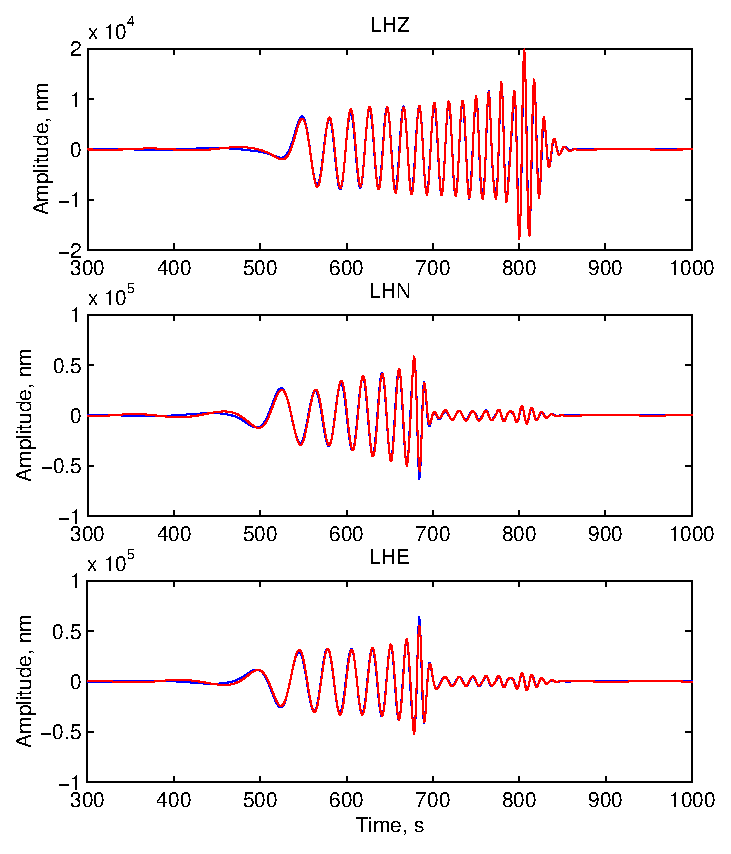
\includegraphics[width=5 in]{Figures/Fig1a}
\caption{Station BJT. Comparison with Herrmann's plane code. 
Three-component synthetic seismogram for the fundamental spheroidal and toroidal modes. 
{\bf Mineos} seismogram is plotted in red, Herrmann's in blue. Earthquake is 
25.39N, 101.40E (Southern China), depth is 33 km. Model is 
PREM, in which the water layer is filled with the upper crust's velocities.
The crust has only two layers.
}
\label{fig:1a}
\end{center}
\end{figure}
%Figure 2
\begin{figure}
\begin{center}
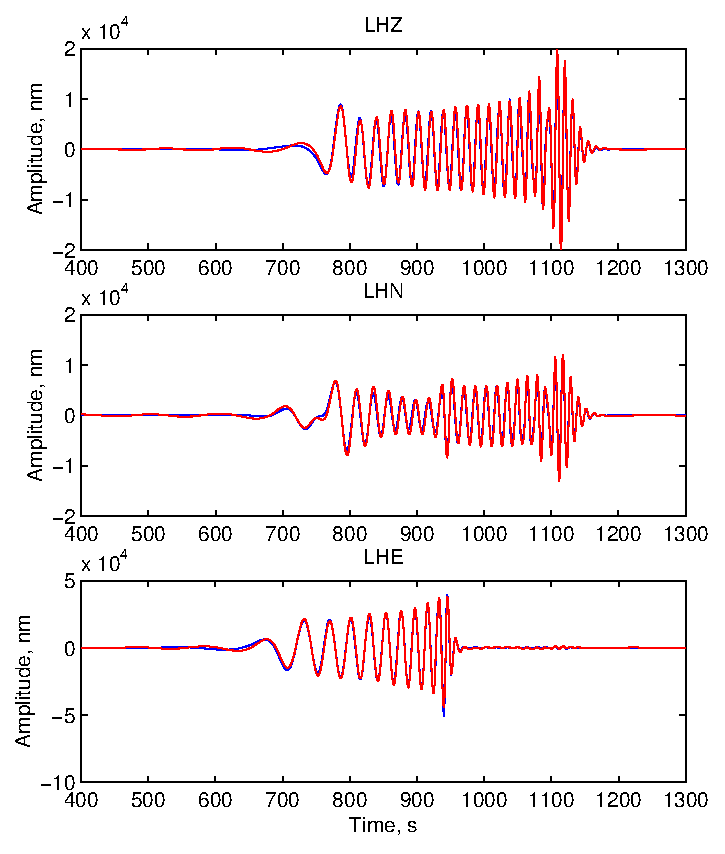
\includegraphics[width=5 in]{Figures/Fig2a}
\caption{Comparison with Herrmann's plane code, as in Figure \ref{fig:1a}, but for 
station TLY.} 
\label{fig:2a}
\end{center}
\end{figure}
%Figure 3
\begin{figure}
\begin{center}
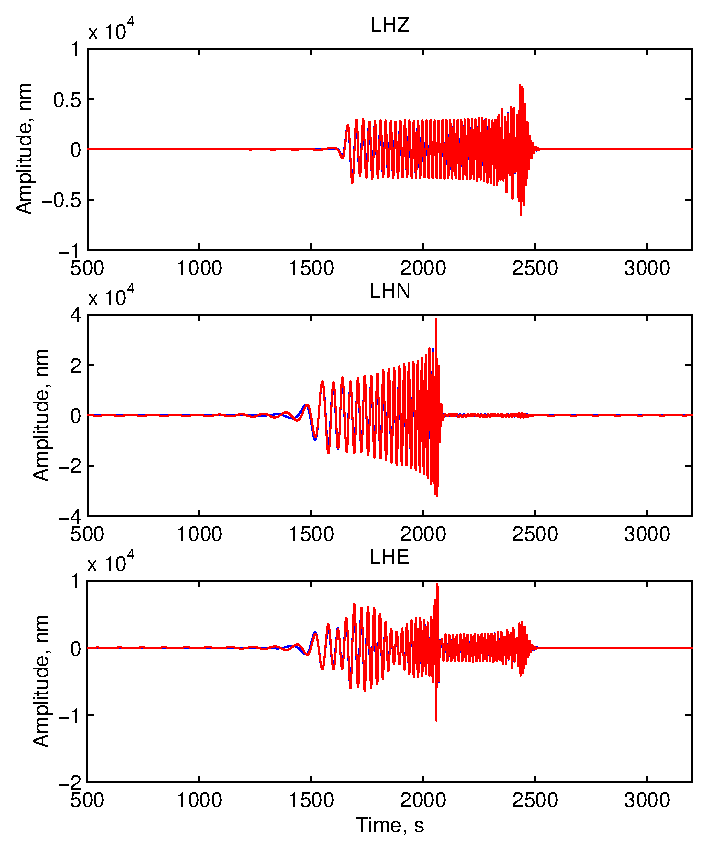
\includegraphics[width=5 in]{Figures/Fig3a}
\caption{Comparison with Herrmann's plane code, as in Figure \ref{fig:1a}, but for 
station BILL.} 
\label{fig:3a}
\end{center}
\end{figure}
%Figure 4
\begin{figure}
\begin{center}
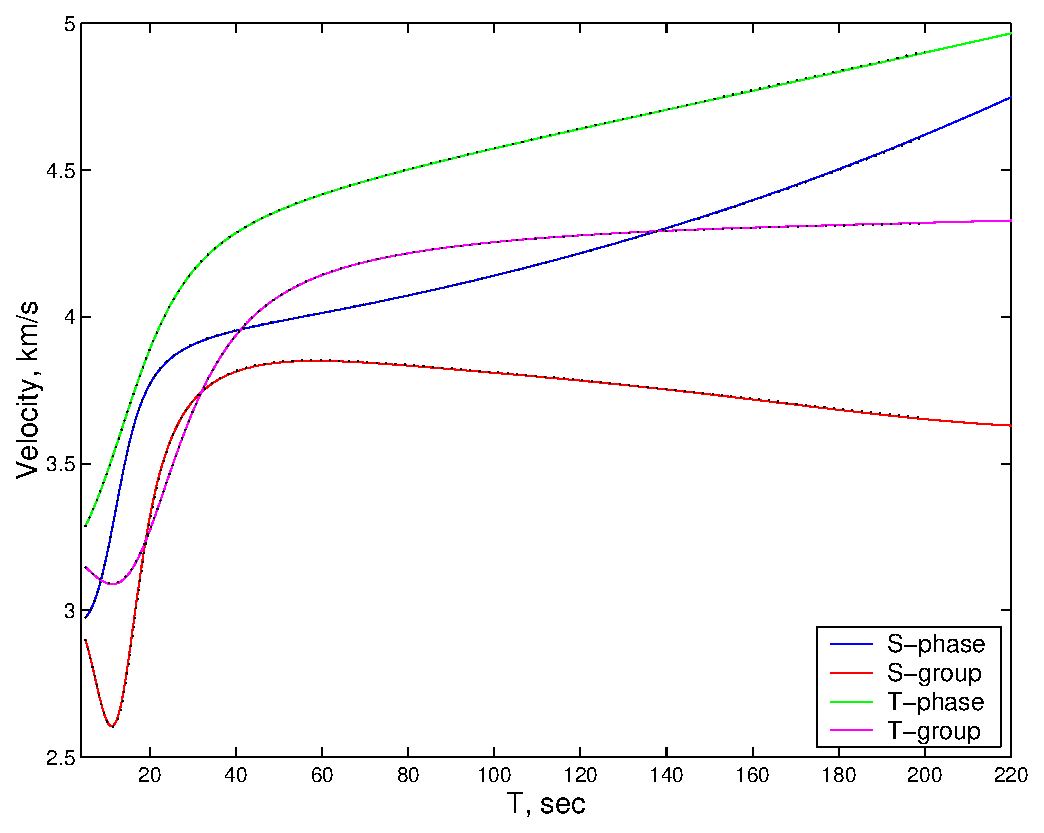
\includegraphics[width=5 in]{Figures/Fig4a}
\caption{Dispersion curves of phase and group velocities for spheroidal and totoidal
fundamental modes. The solid color lines are the {\bf Mineos} results, the 
black dotted lines are for the Herrmann's plane code. The solid lines 
color are: blue for Rayleigh phase velocity, red for Rayleigh group 
velocity, green for Love phase velocity, and magneta for group Love velocity. }
\label{fig:4a}
\end{center}
\end{figure}
% MINEOS VS SPECFM
%
\newpage
\subsection{Benchmark test \#3. Mineos vs SPECFEM3D\_GLOBE}

The  {\bf Mineos} synthetic seismograms were tested against SPECFEM3D\_GLOBE
synthetic seismograms for the same event and station set as described in 
the previous section.

\noindent \textbf{\emph{Input 1D model.}} The input model is an anisotropic, 
single-layered crust
PREM with attenuation. The 3 km water layer is filled with crustal properties.
SPECFEM3D\_GLOBE has a special subroutine for evaluation of the model parameters by 
polynomial interpolation across a fixed number of layers from the center of
the Earth up to the free surface at radius 6371 km. This polynomial 
representation was converted by a special program to a plain input file in
{\bf Mineos} format. The total number of vertical nodes is 237. The tabulated
step by depth in the crust and upper mantle is close to 1 km.

\noindent \textbf{\emph{SPECFEM3D\_GLOBE run notes.}} SPECFEM3D\_GLOBE  was configured to make
the synthetic seismogram (displacement, nm) 1 hour long. The Earth was split
into 6 chunks. Each chunk consisted of ~480x480 elements.
So, the average lateral size of the elements near to the surface was ~20x20 km.
The state of some important run parameters were: ELLIPTICITY - off,
TOPOGRAPHY - off, ROTATION - off, and GRAVITY - on. As with {\bf Mineos}, input
coordinates are geographic and geocentric coordinates are used internally.

\noindent \textbf{\emph{Mineos run notes.}} {\bf Mineos} was configured to compute all normal modes
in the frequency range $0 - 0.2$ Hz and the radial mode range $0 \le n \le 400$. 
In total, the program computed 247565 spheroidal normal modes, 162154 toroidal modes, and 
240 radial modes. Synthetic seismograms (acceleration, nm/s$^2$) 1 hour long 
were simulated. All seismograms were converted from acceleration to 
displacement in nm.

\noindent \textbf{\emph{Tapering, results discussion.}} To reduce noise at 
spectral edges, all seismograms  were half cosine tapered with corner 
frequencies $(1/200,\; 1/100)$ Hz and $(1/12, \;1/10)$ Hz.
Figures \ref{fig:5a} - \ref{fig:16a} illustrate three-component seismograms and amplitude spectra
for the BJT, TLY, and BILL stations. SPECFEM3D\_GLOBE results are plotted 
in red, {\bf Mineos} in blue.

\noindent The test shows that synthetic seismograms and spectra 
for both methods are close. Attempts to increase the high cut
frequency, say to 5 sec, lead to differences in some places with periods 
close to 8 sec. This probably resulted because the SPECFEM3D\_GLOBE spectral 
elements were not small enough.

% Station BJT

%Figure 5
\begin{figure}
\begin{center}
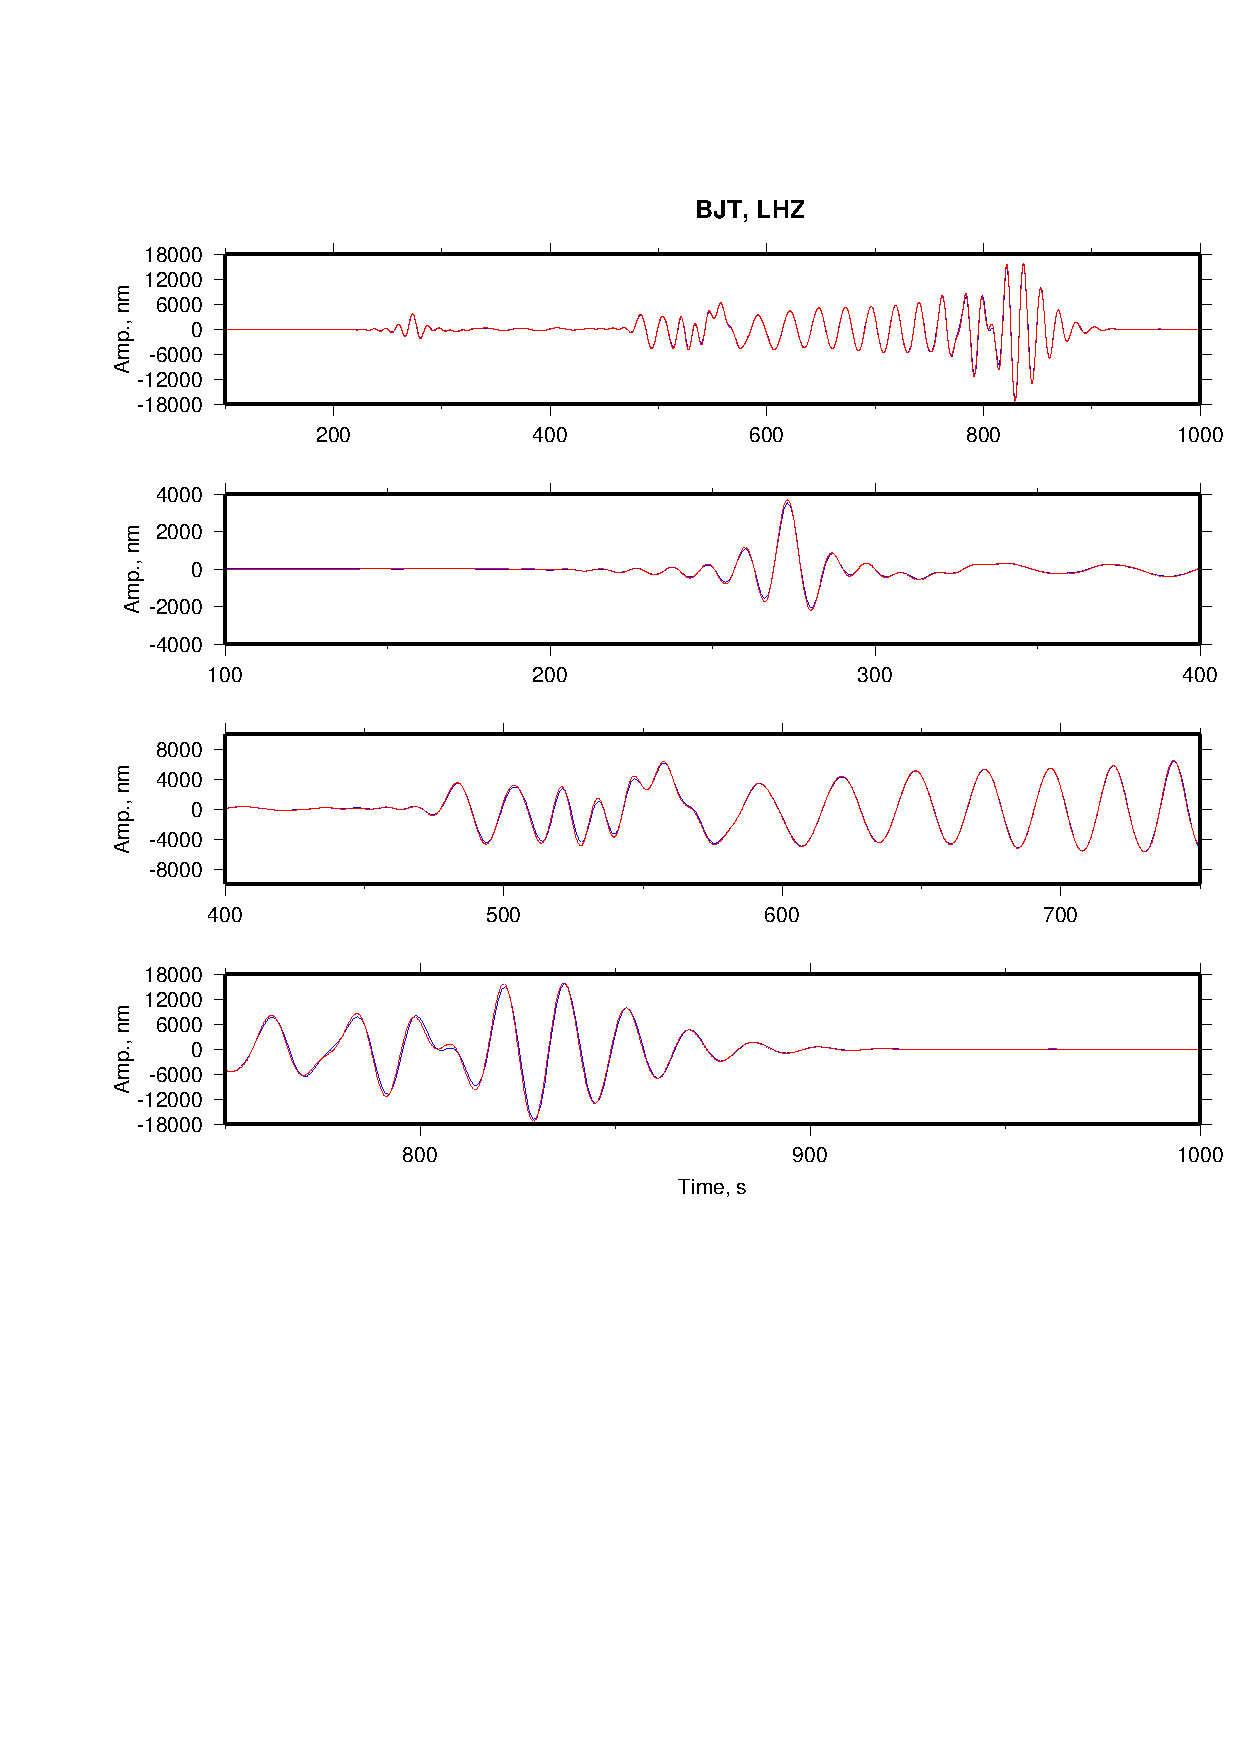
\includegraphics[width=7 in]{Figures/FigsBJTLHZ}
\caption{Synthetic seismograms for SPECFEM3D\_GLOBE (red) and {\bf Mineos} (blue). Station BJT, chan LHZ. 
Distance = $19.123^o$, Az = $-135.267^o$.
The top plot shows the whole record, the others plot separate fragments. }
\label{fig:5a}
\end{center}
\end{figure}

%Figure 6
\begin{figure}
\begin{center}
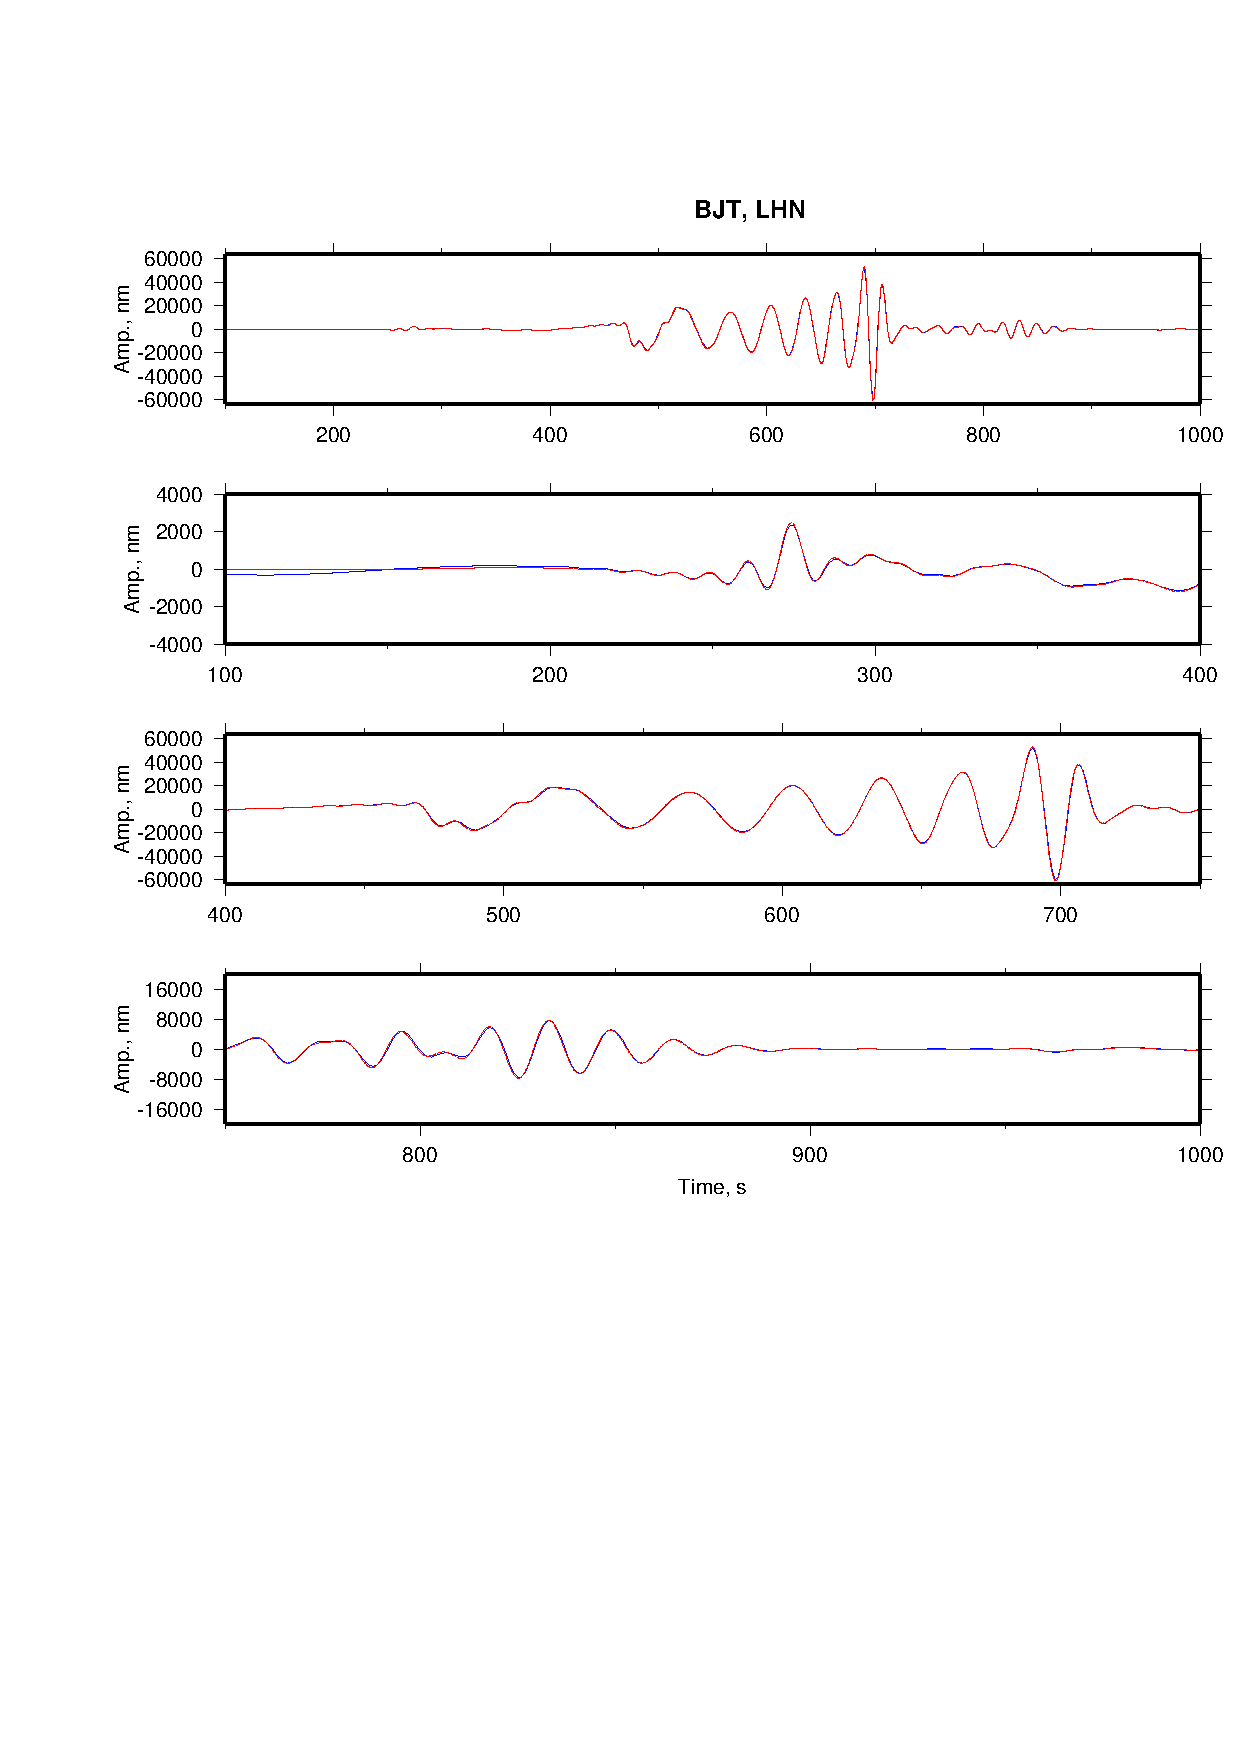
\includegraphics[width=7 in]{Figures/FigsBJTLHN}
\caption{ The same as Figure \ref{fig:5a}, but for LHN channel.}
\label{fig:6a}
\end{center}
\end{figure}

%Figure 7
\begin{figure}
\begin{center}
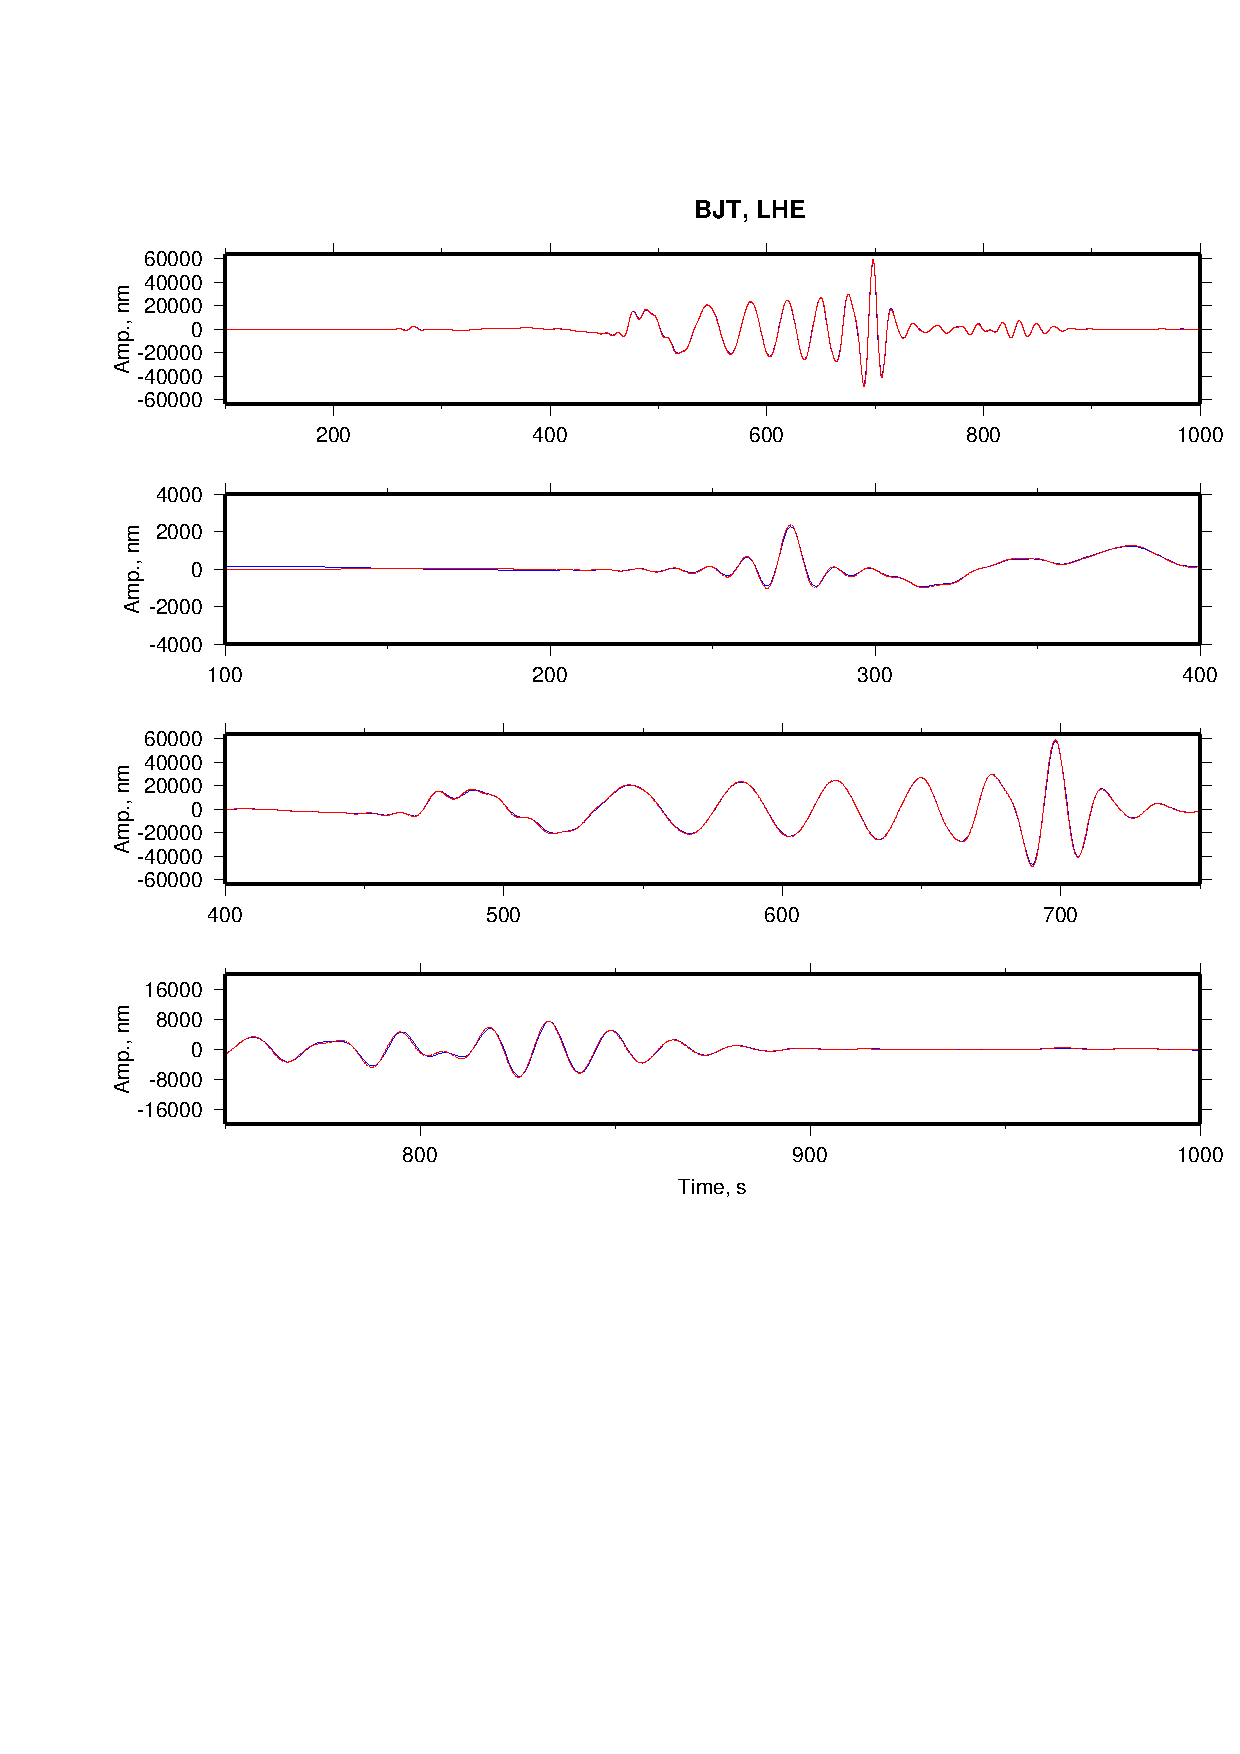
\includegraphics[width=7 in]{Figures/FigsBJTLHE}
\caption{The same as Figure \ref{fig:5a}, but for LHE channel.}
\label{fig:7a}
\end{center}
\end{figure}

%Figure 8
\begin{figure}
\begin{center}
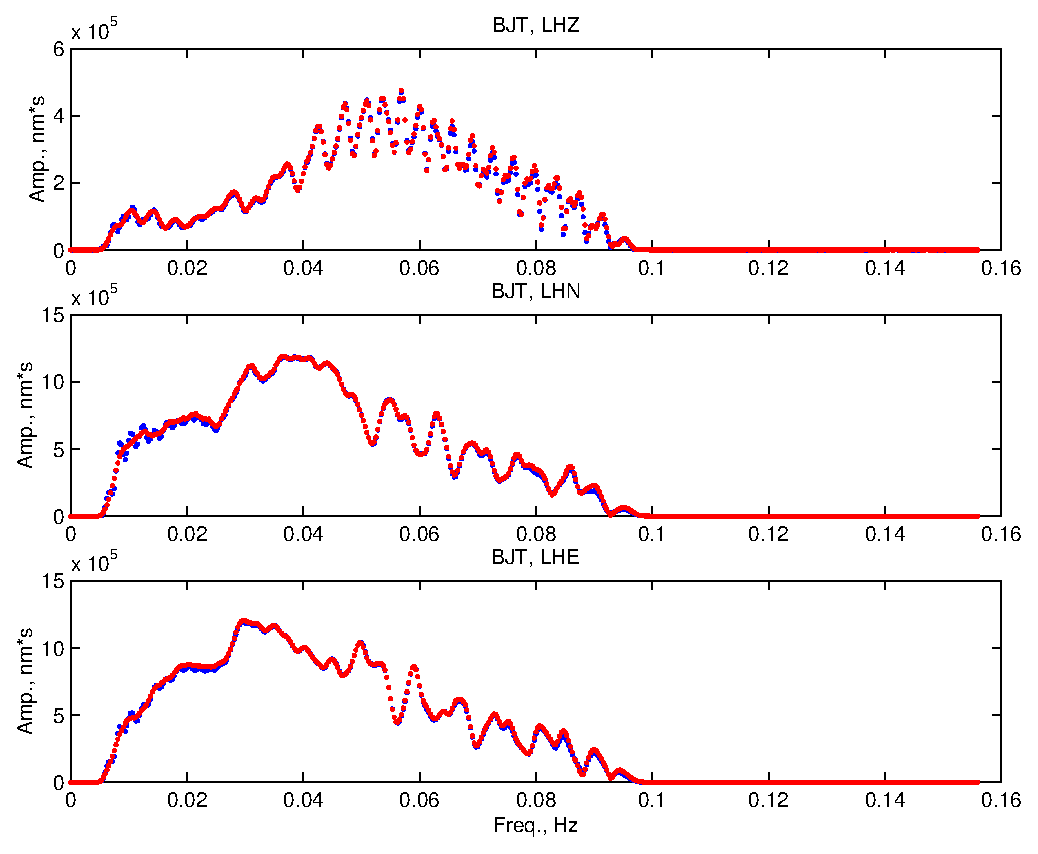
\includegraphics[width=7 in]{Figures/FspBJT}
\caption{Amplitude spectra for the station BJT. Red color - SPECFEM3D\_GLOBE spectra, blue - {\bf Mineos}.}
\label{fig:8a}
\end{center}
\end{figure}

% Station TLY 

%Figure 9
\begin{figure}
\begin{center}
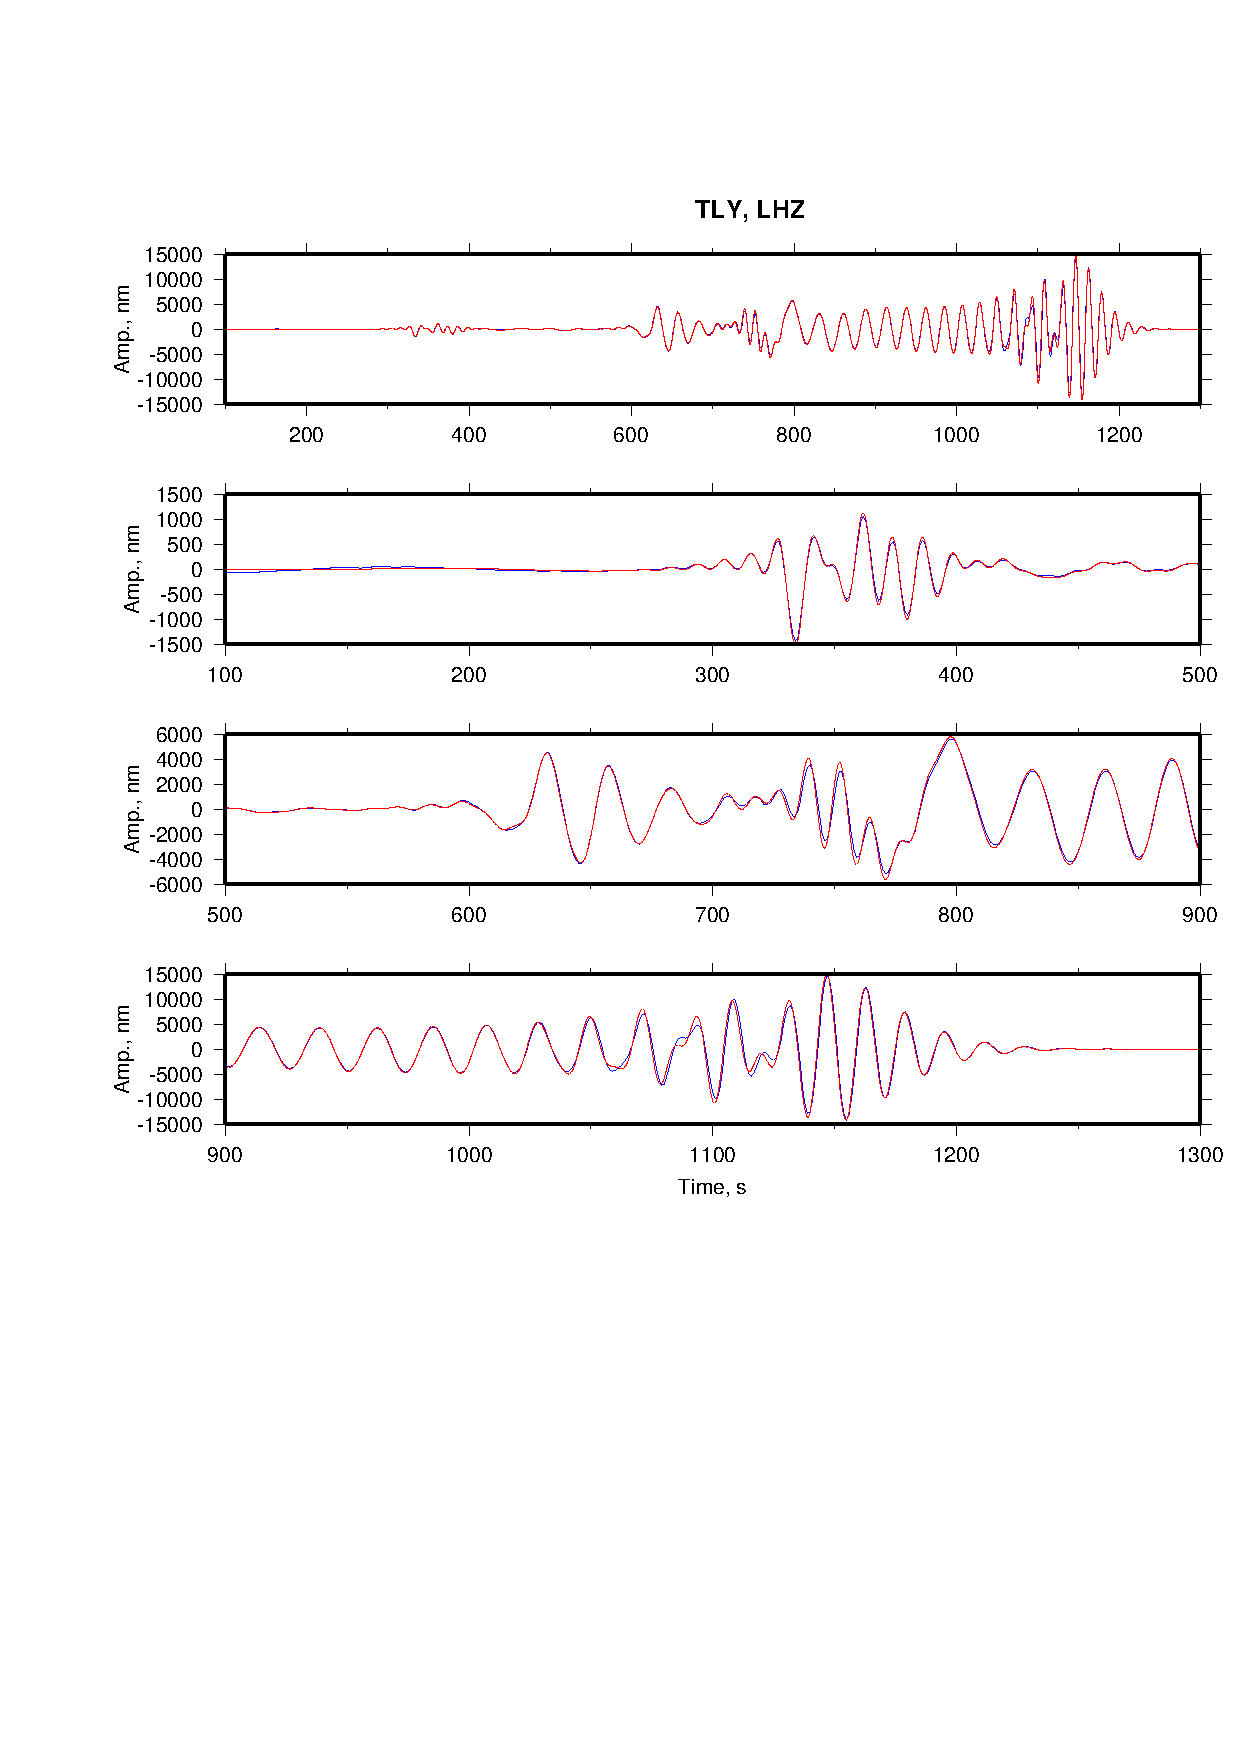
\includegraphics[width=7 in]{Figures/FigsTLYLHZ}
\caption{Synthetic seismograms for SPECFEM3D\_GLOBE (red) and {\bf Mineos} (blue). Station TLY, chan LHZ. 
Distance = $26.308^o$, Az = $-175,417^o$.
The top plot shows the whole record, the others plot separate fragments. }
\label{fig:9a}
\end{center}
\end{figure}

%Figure 10
\begin{figure}
\begin{center}
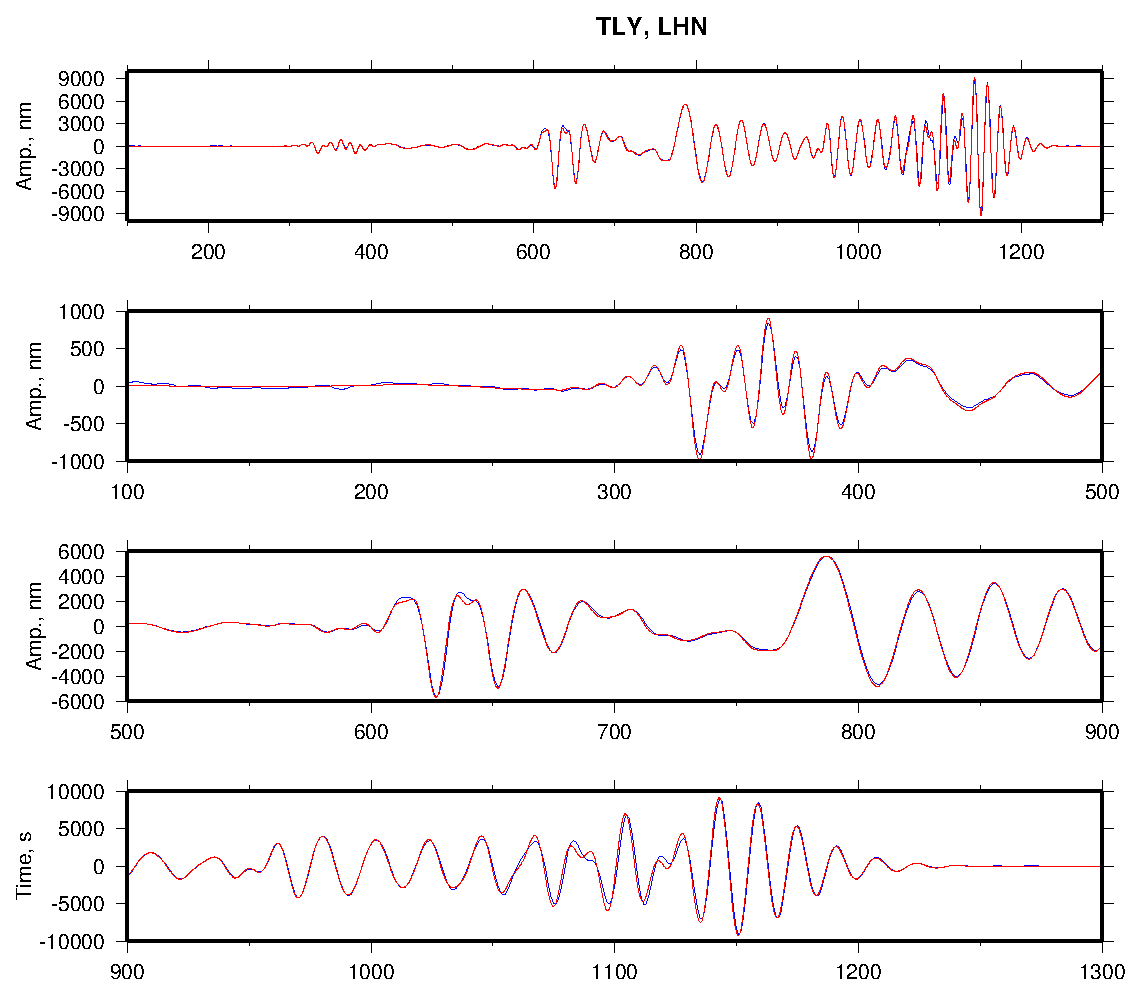
\includegraphics[width=7 in]{Figures/FigsTLYLHN}
\caption{ The same as Figure \ref{fig:9a}, but for LHN channel.}
\label{fig:10a}
\end{center}
\end{figure}

%Figure 11
\begin{figure}
\begin{center}
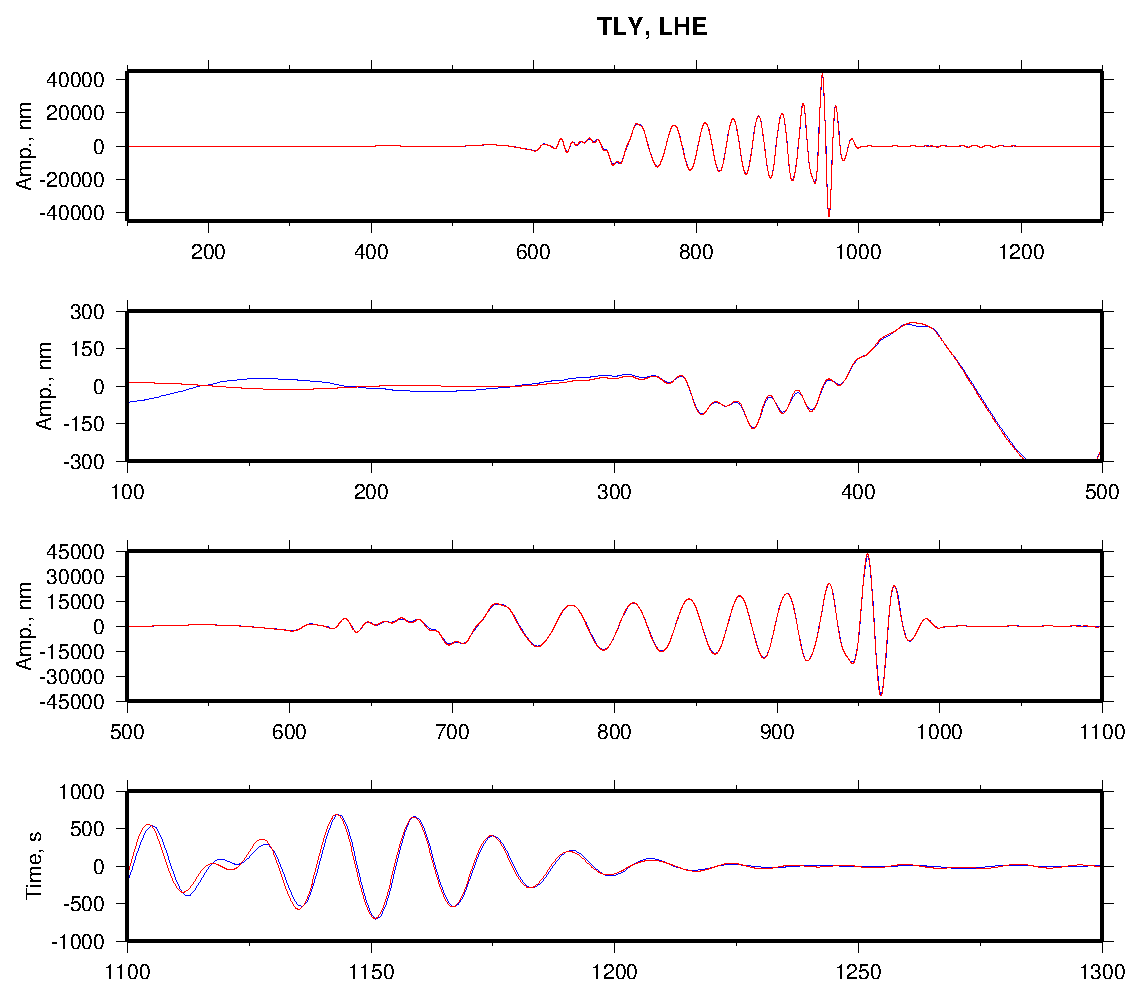
\includegraphics[width=7 in]{Figures/FigsTLYLHE}
\caption{ The same as Figure \ref{fig:9a}, but for LHE channel.}
\label{fig:11a}
\end{center}
\end{figure}

%Figure 12
\begin{figure}
\begin{center}
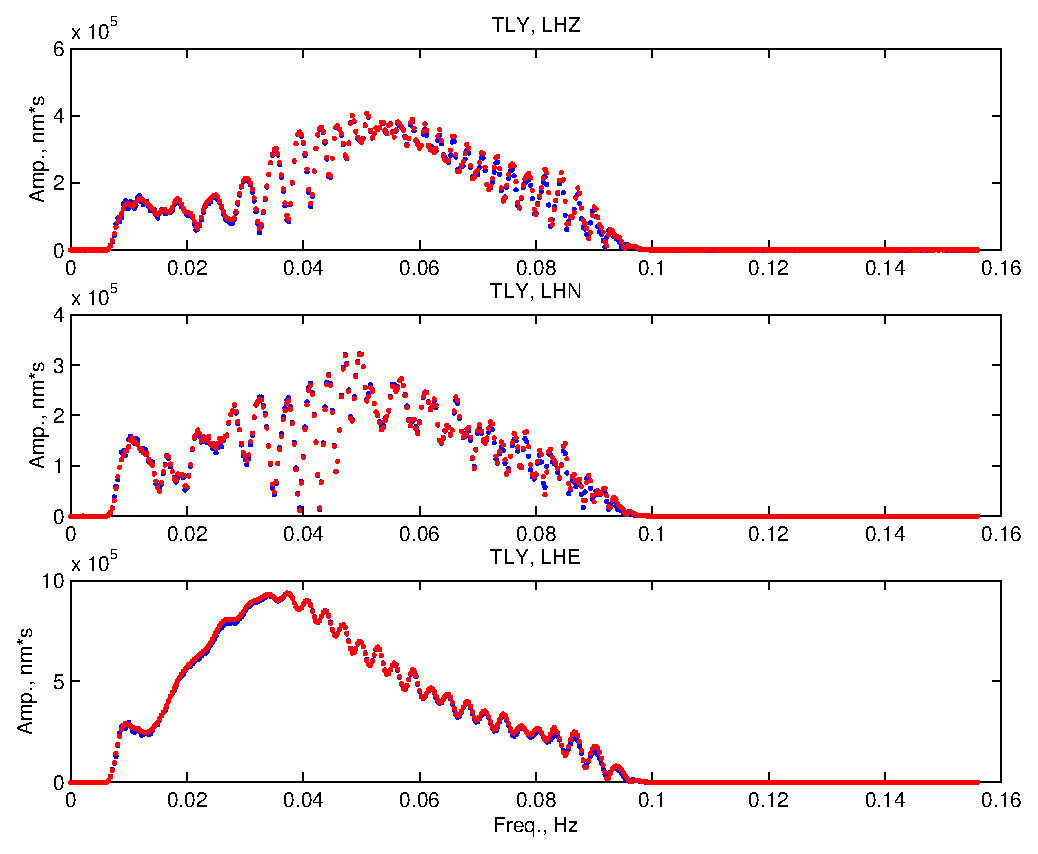
\includegraphics[width=7 in]{Figures/FspTLY}
\caption{Amplitude spectra for the station TLY. Red color - SPECFEM3D\_GLOBE spectra, blue - {\bf Mineos}.}
\label{fig:12a}
\end{center}
\end{figure}

% Station BILL

%Figure 13
\begin{figure}
\begin{center}
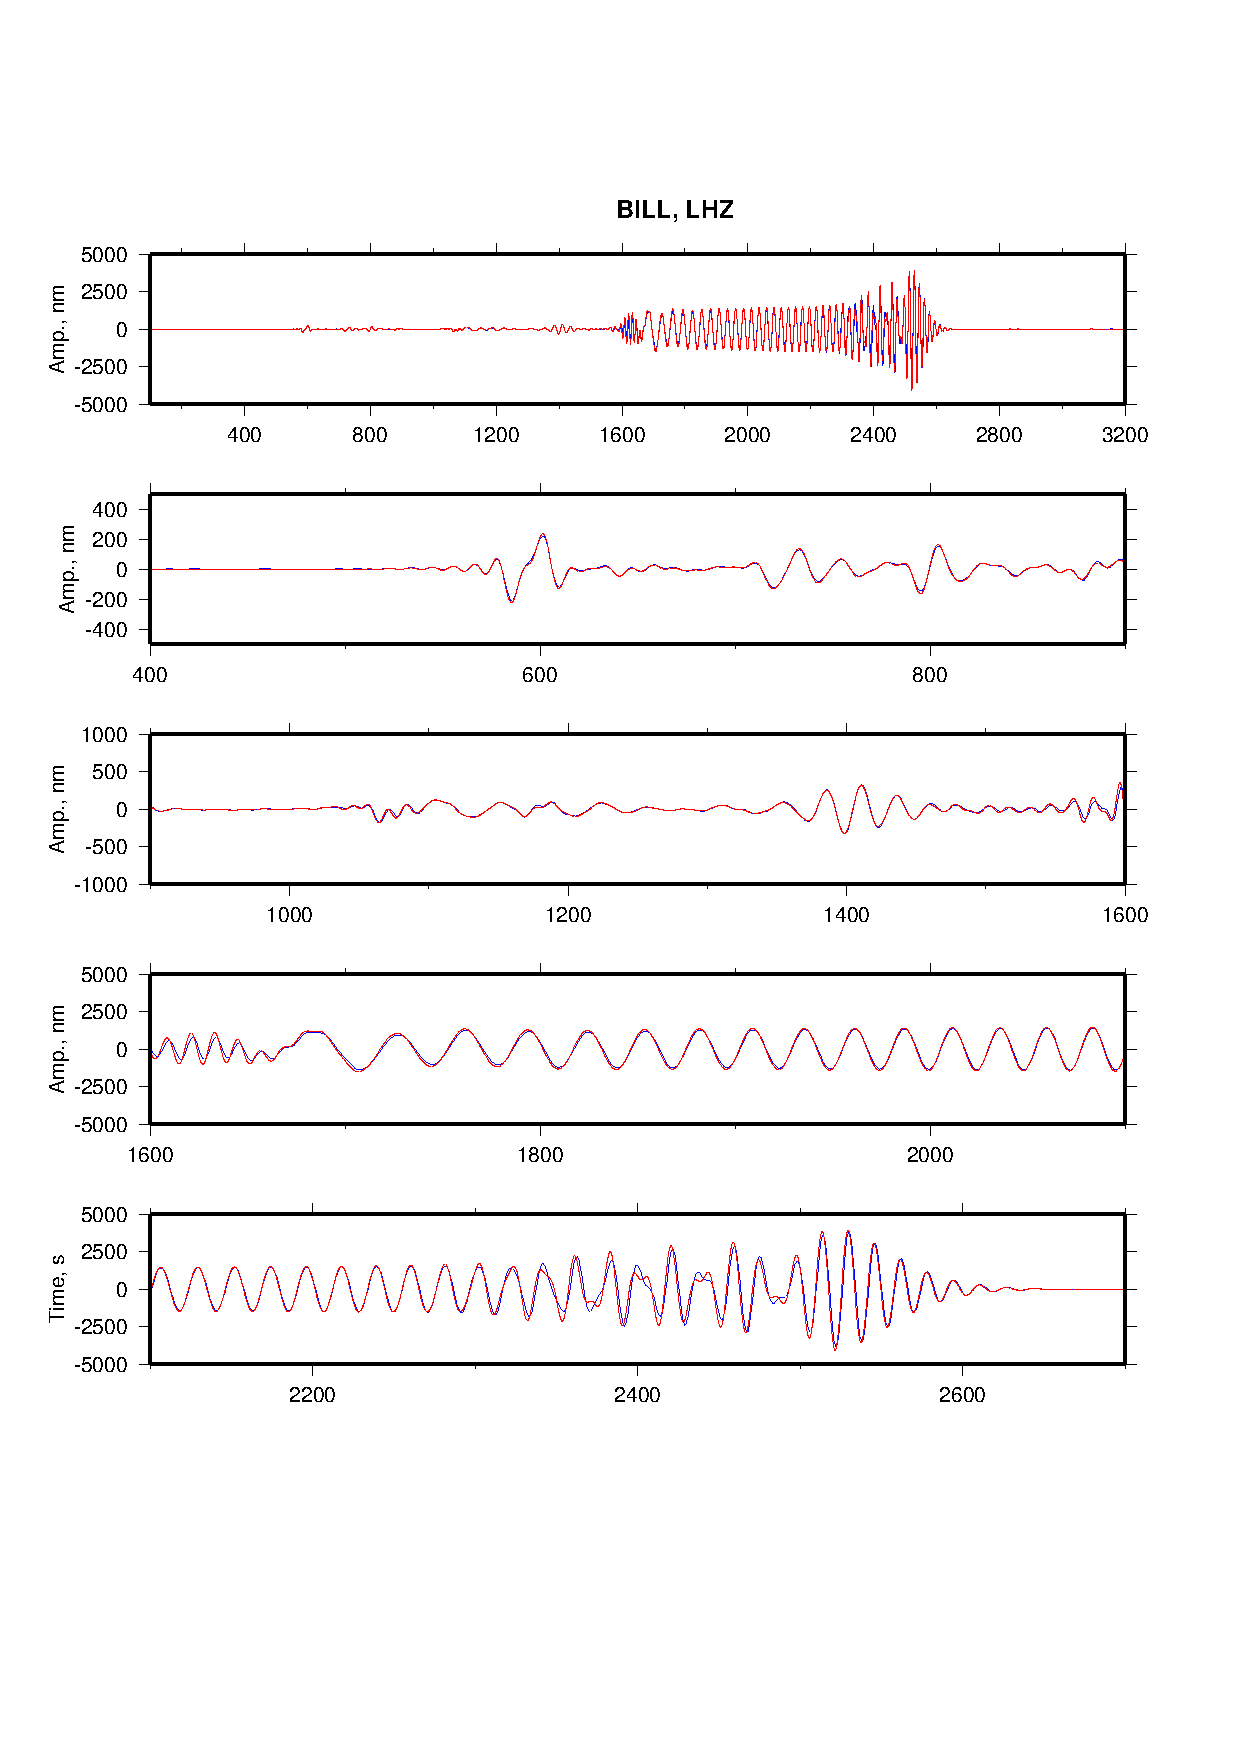
\includegraphics[width=7 in]{Figures/FigsBILLLHZ}
\caption{Synthetic seismograms for SPECFEM3D\_GLOBE (red) and {\bf Mineos} (blue). Station BILL, chan LHZ. 
Distance = $57.417^o$, Az = $-103.266^o$.
The top plot shows the whole record, the others plot separate fragments. }
\label{fig:13a}
\end{center}
\end{figure}

%Figure 14
\begin{figure}
\begin{center}
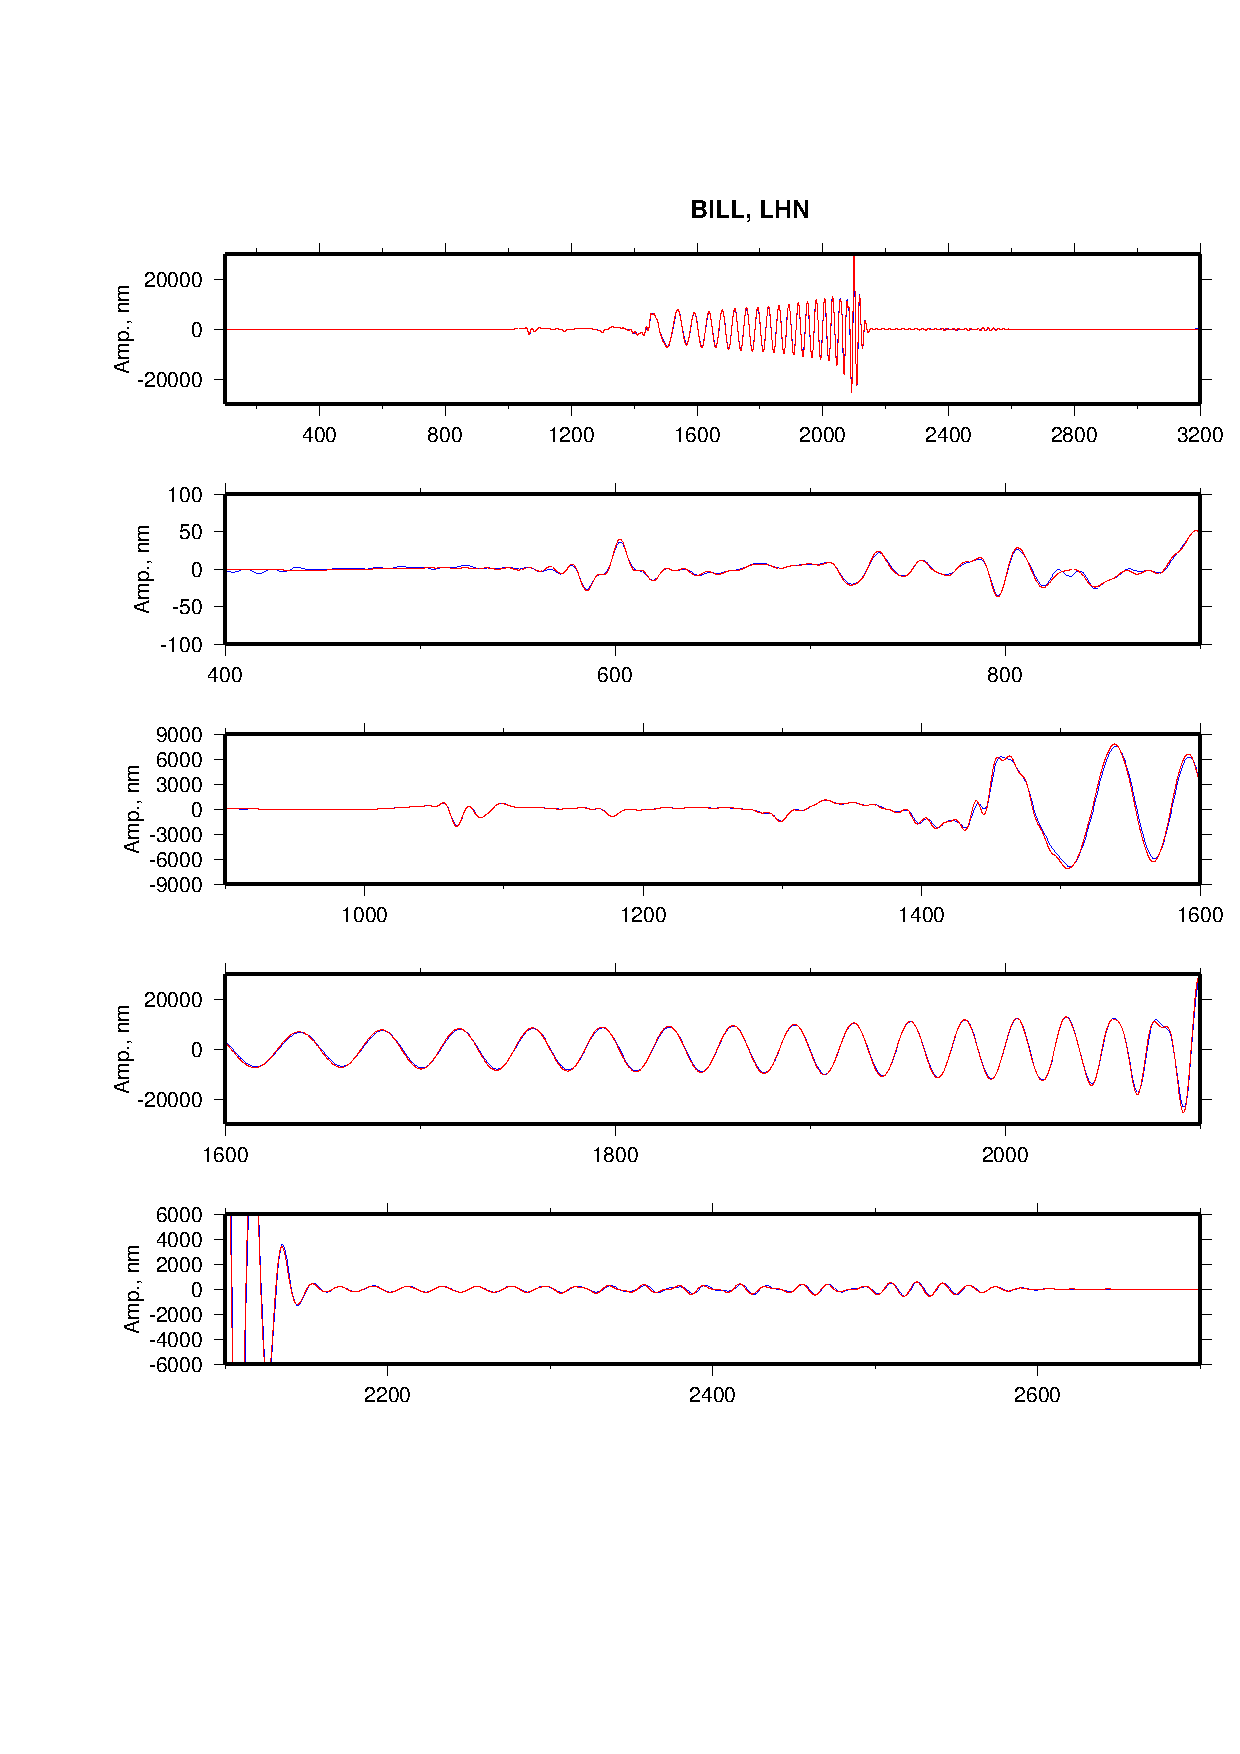
\includegraphics[width=7 in]{Figures/FigsBILLLHN}
\caption{ The same as Figure \ref{fig:13a}, but for LHN channel.}
\label{fig:14a}
\end{center}
\end{figure}

%Figure 15
\begin{figure}
\begin{center}
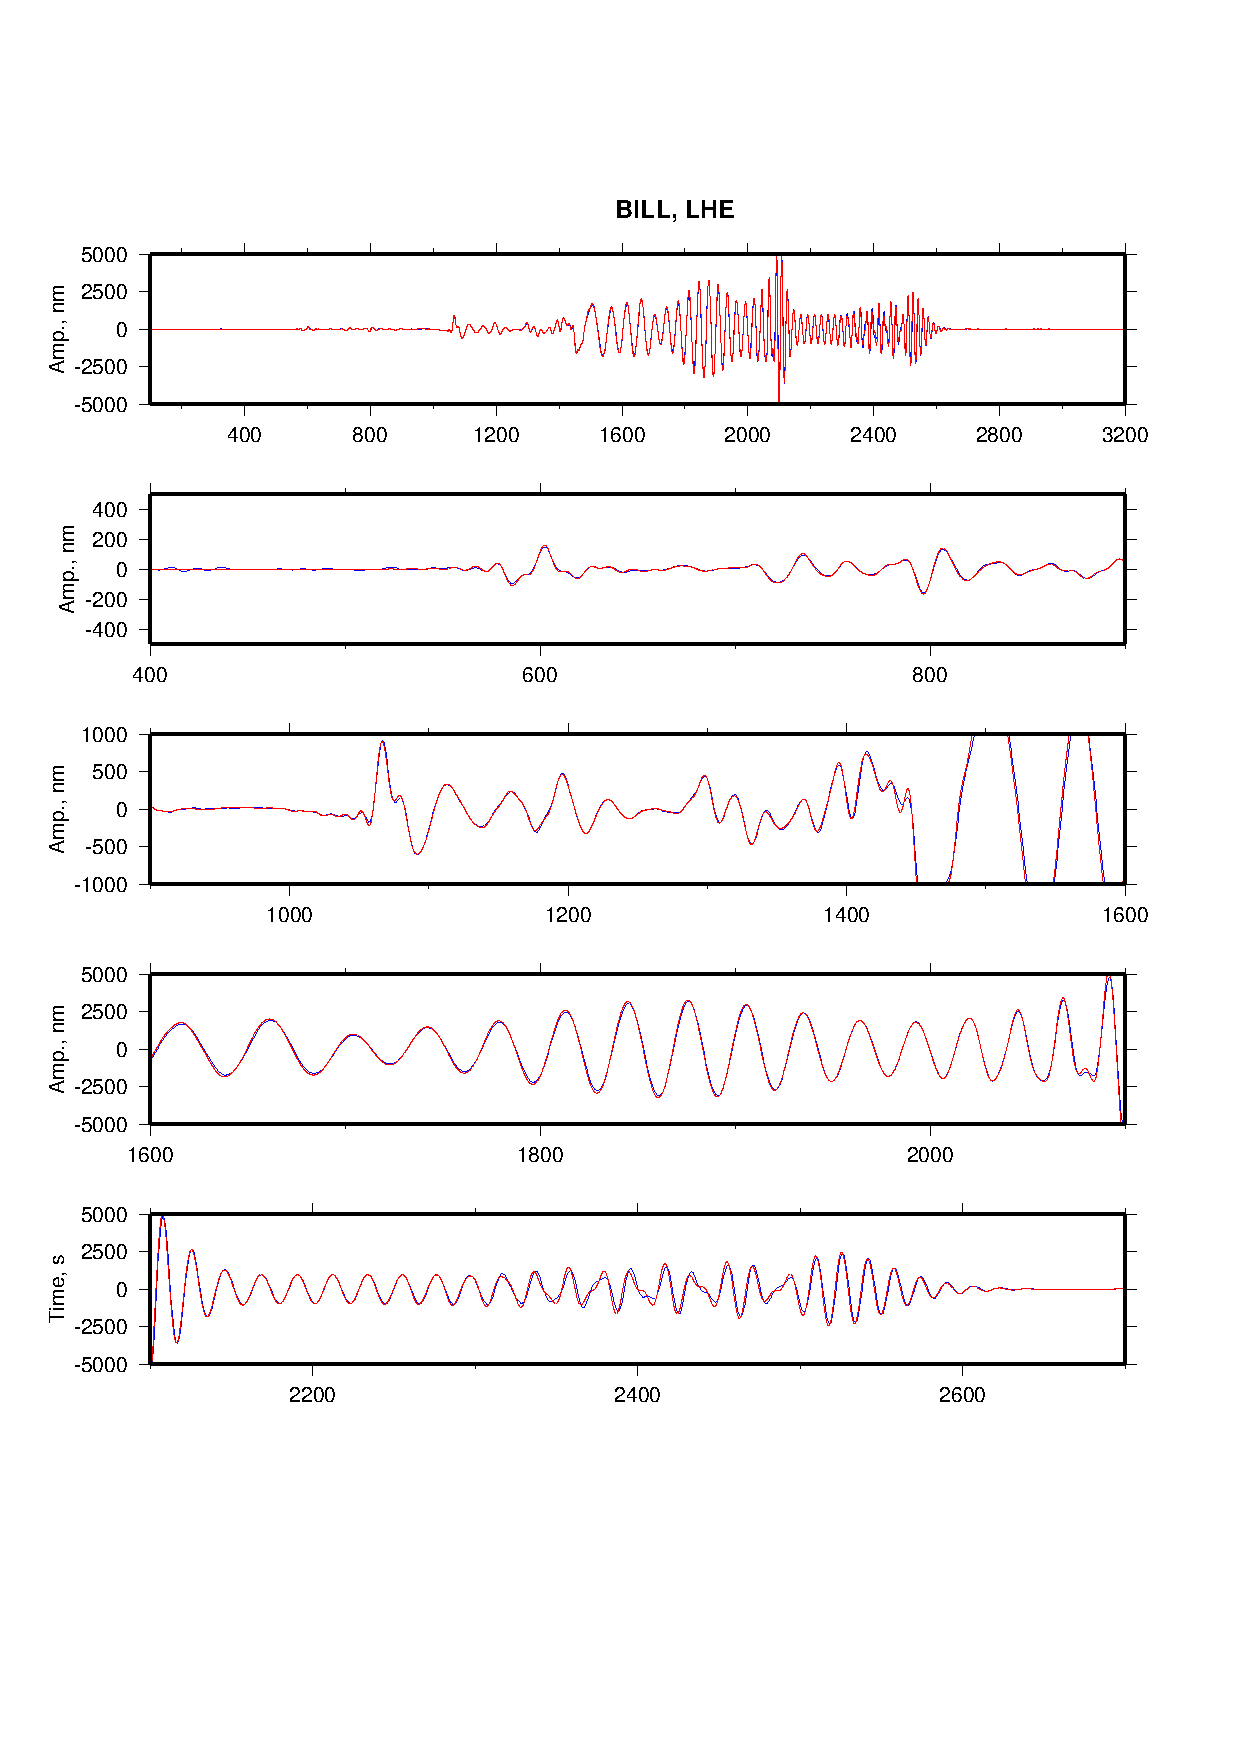
\includegraphics[width=7 in]{Figures/FigsBILLLHE}
\caption{ The same as Figure \ref{fig:13a}, but for LHE channel.}
\label{fig:15a}
\end{center}
\end{figure}

%Figure 16
\begin{figure}
\begin{center}
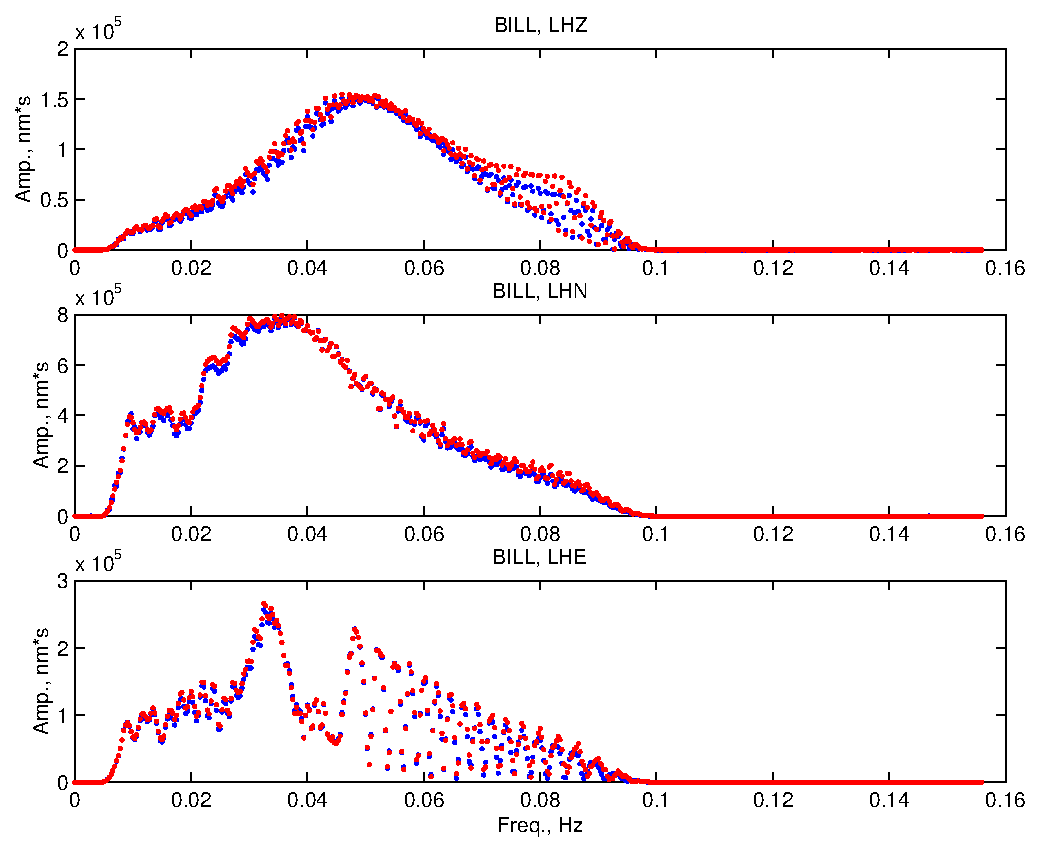
\includegraphics[width=7 in]{Figures/FspBILL}
\caption{Amplitude spectra for the station BILL. Red color - SPECFEM3D\_GLOBE spectra, blue - {\bf Mineos}.}
\label{fig:16a}
\end{center}
\end{figure}

